\documentclass[crop,class=article]{standalone}
%----------------------------Preamble-------------------------------%
\usepackage{amssymb}
\usepackage{tikz}                       % Drawing/graphing tools.
\usetikzlibrary{arrows.meta}            % Latex and Stealth arrows.
\DeclareMathSymbol{\minus}{\mathbin}{AMSa}{"39} % Unary minus sign.
%--------------------------Main Document----------------------------%
\begin{document}
    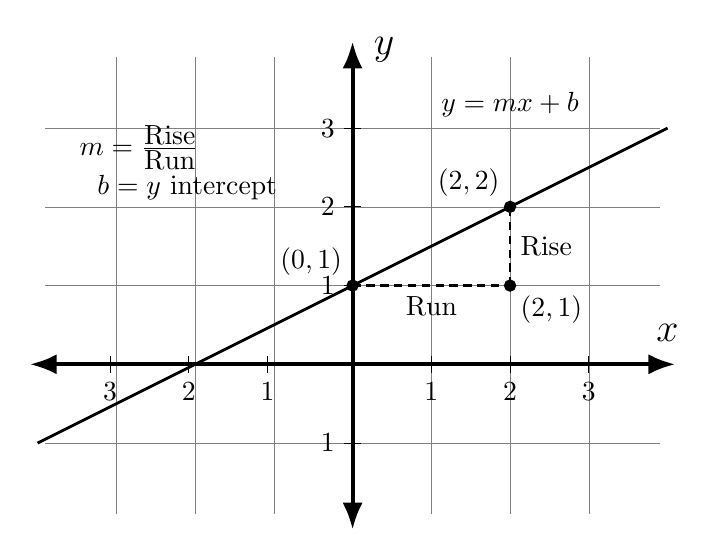
\begin{tikzpicture}[>=latex, line width=1pt]
        \draw[style=help lines] (-3.9, -1.9) grid (3.9, 3.9);
        \begin{scope}[line width=0.3pt]
            \foreach\n in {1,2,3}{%
                \draw (\n,3pt) -- (\n,-3pt) node [below] {$\n$};
                \draw (3pt,\n) -- (-3pt,\n) node [left] {$\n$};
                \draw (-\n.08,3pt) -- (-\n.08,-3pt) node [below] {$\minus\n$};
            }
            \draw (3pt,-1) -- (-3pt,-1) node [left] {$\minus{1}$};
        \end{scope}
        \begin{scope}[line width=1.5pt, >=Latex, font=\Large]
            \draw[<->] (-4.1, 0) to (4.1, 0);
            \draw[<->] (0, -2.1) to (0, 4.1);
            \node at (4, 0.4) {$x$};
            \node at (0.4, 4) {$y$};
        \end{scope}
        \draw (-4, -1) to (4, 3);
        \draw[fill=black] (0,1) circle (0.6mm) node[above left] {$(0,1)$};
        \draw[fill=black] (2,2) circle (0.6mm) node[above left] {$(2,2)$};
        \draw[fill=black] (2,1) circle (0.6mm) node[below right] {$(2,1)$};
        \draw[densely dashed] (0,1) to node [below] {Run} (2,1);
        \draw[densely dashed] (2,1) to node [right] {Rise} (2,2);
        \node at (-2.71,2.75) {$m=\frac{\textrm{Rise}}{\textrm{Run}}$};
        \node at (-2.1,2.25) {$b=y\textrm{ intercept}$};
        \node at (2,3.3) {$y=mx+b$};
    \end{tikzpicture}
\end{document}